\section{Детектирование нахождения в опасной зоне}
\begin{frame}
    \frametitle{Простейшее определение опасной зоны}
    В простейшем случае, опасную зону можно определить следующим образом.

    Зафиксируем выпуклый многоугольник $A$ на изображении.
    $$ x_{min} = \min\{ x : \exists y (x, y) \in A\} $$
    $$ x_{max} = \max\{ x : \exists y (x, y) \in A\} $$

    Тогда опасной зоной $DZ$ будем называть выпуклую оболочку множества
    $$ A \cup \{(x_{min}, 0), (x_{max}, 0)\} $$
\end{frame}

\begin{frame}
    \frametitle{Определение принадлежности опасной зоне}
    Задан минимальный порог срабатывания $m$ для принадлежности ключевой точки зоне.

    По определению $I_i = 1$, если ключевая точка человека $\left(x_i, y_i, c_i\right)$ находится в опасной зоне.
    $$ I_i = 1 \iff \left(c_i \ge m\right) \wedge \left(\left(x_i, y_i\right) \in DZ\right) $$

    Задана минимальная доля $t$ ключевых точек, принадлежащих опасной зоне, при которой считаем человека находящимся в ней.

    Считаем, что человек находится в опасной зоне, если:
    $$ \frac{\sum I_i}{N} \ge t $$
\end{frame}

\begin{frame}
    \frametitle{Усложнение определения опасной зоны}
    Будем считать, что область пространства, обозреваемого камерой, локально представляет из себя $\mathbb{R}^3$.

    Зафиксируем правильный многоугольник $A$ в плоскости $z = 0$.
    Тогда опасной зоной будем называть множество:
    $$DZ = \{(x, y, z) : (x, y, 0) \in A\} $$
\end{frame}

\begin{frame}
    \frametitle{Детектирование нахождения в опасной зоне}
    \begin{figure}
        \centering
        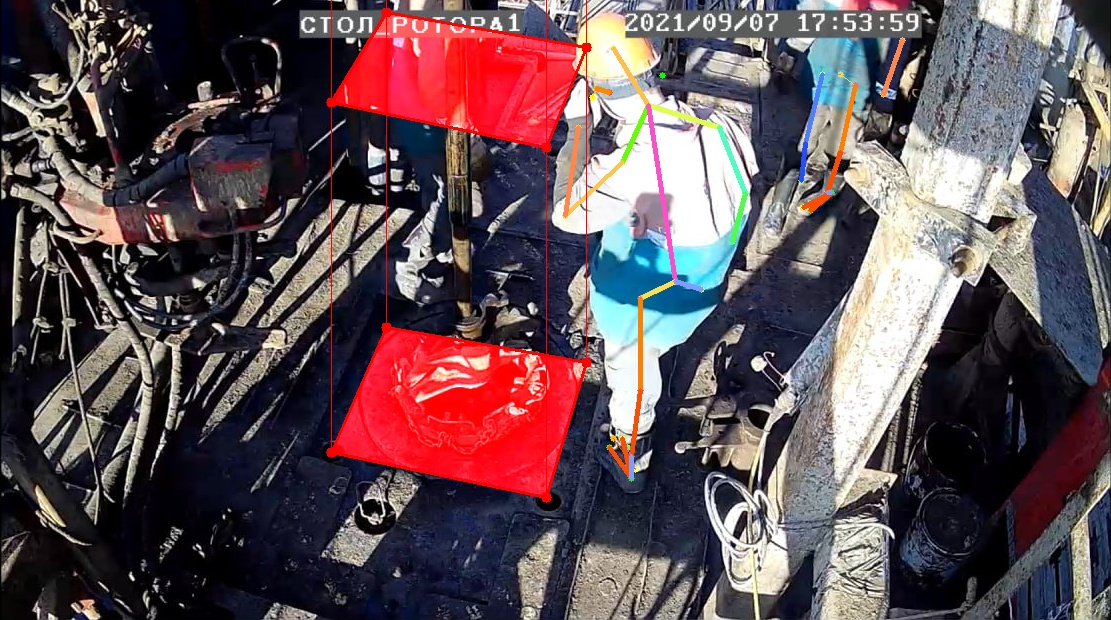
\includegraphics[width=1.0\textwidth,keepaspectratio]{danger_zone}
    \end{figure}
\end{frame}

\begin{frame}
    \frametitle{Оценка расстояния до объектов}
    Рассмотренные подходы к оценке расстояния до объектов:
    \begin{itemize}
        \item Калибровка камеры;
        \item Анализ геометрии помещения;
        \item Аппроксимация карты глубины.
    \end{itemize}
\end{frame}

\begin{frame}
    \frametitle{Карта глубины}
    \begin{definition}
        Карта глубины --- это изображение, где для каждого пикселя вместо цвета хранится расстояние от него до камеры.
    \end{definition}

    \begin{figure}
        \begin{minipage}[!h]{0.49\linewidth}
            \centering
            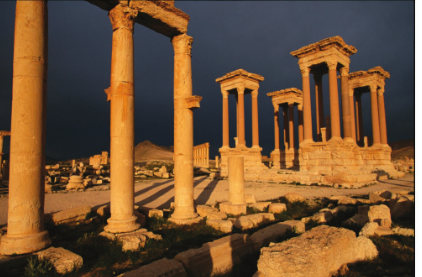
\includegraphics[width=1.0\textwidth,keepaspectratio]{depth_map_example_1}
        \end{minipage}
        \hfill
        \begin{minipage}[!h]{0.49\linewidth}
            \centering
            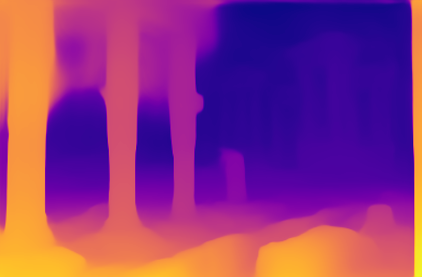
\includegraphics[width=1.0\textwidth,keepaspectratio]{depth_map_example_2}
        \end{minipage}
        \caption{Пример карты глубины, построенной по изображению}
    \end{figure}

\end{frame}

\begin{frame}
    \frametitle{Трёхмерная реконструкция по карте глубины}
    \begin{figure}
        \centering
        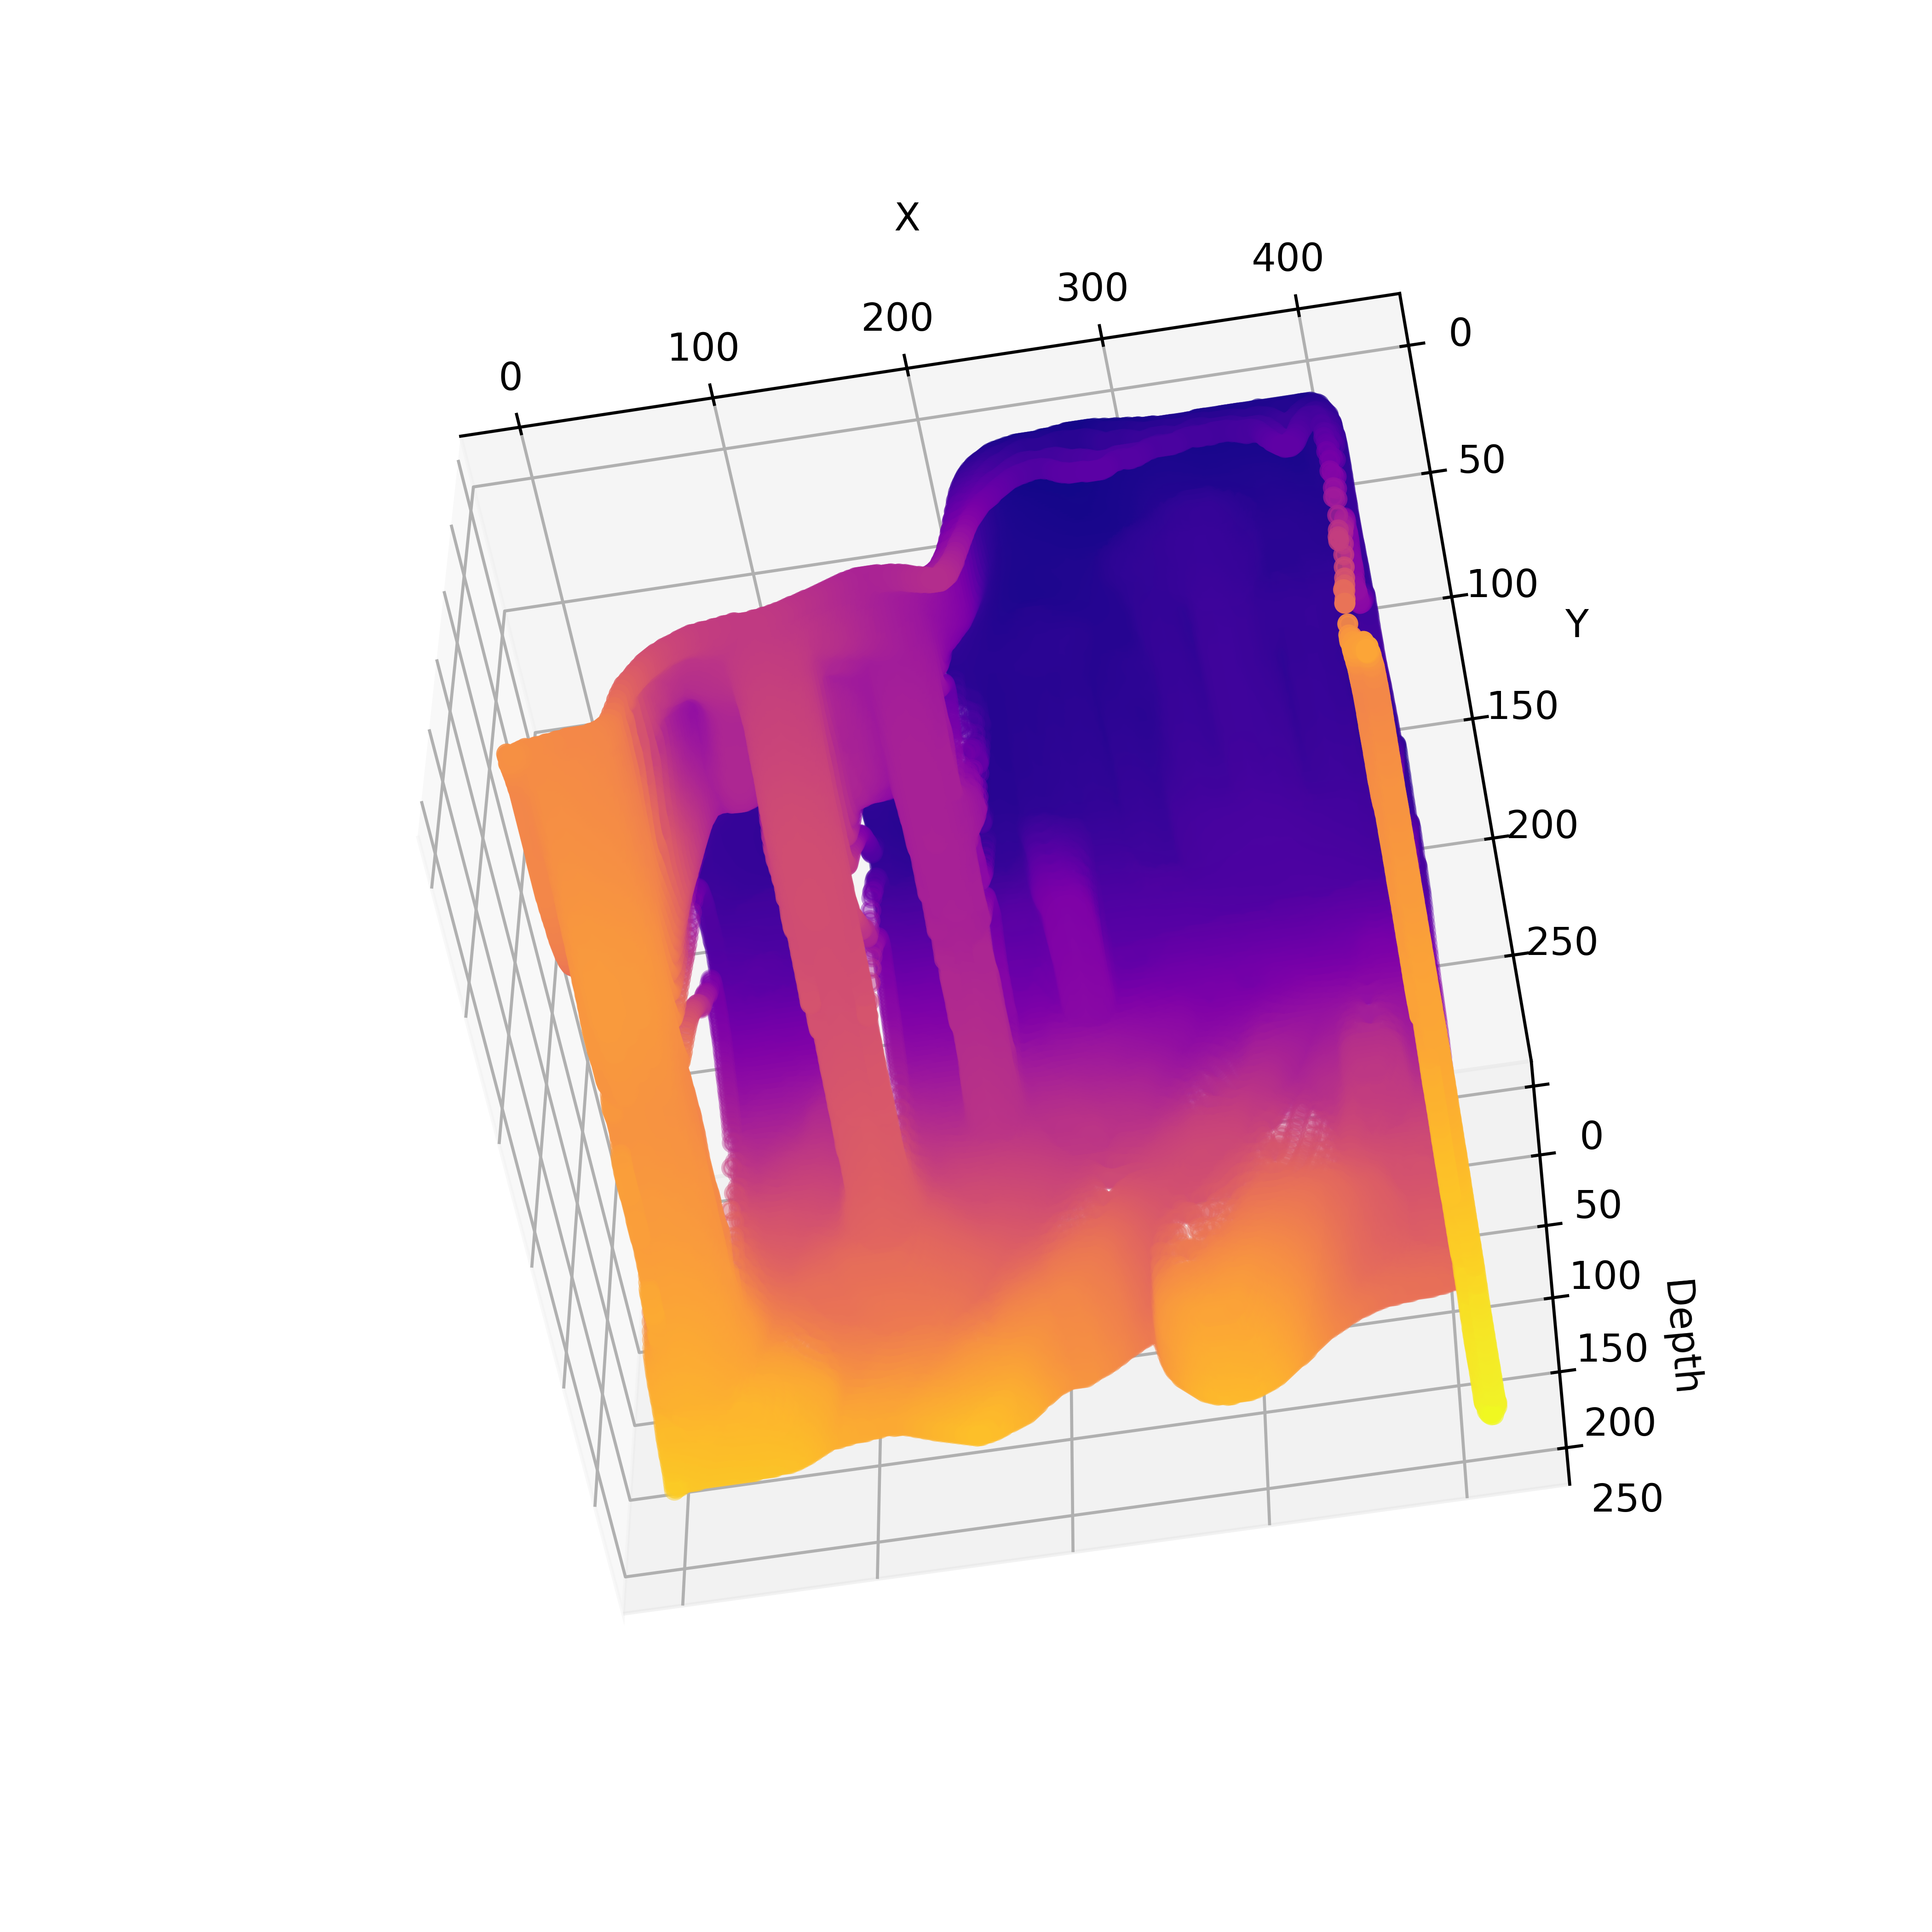
\includegraphics[width=0.8\textwidth,keepaspectratio]{depth_map_example_3}
    \end{figure}
\end{frame}

\begin{frame}
    \frametitle{Модель MiDaS}
    \begin{figure}
        \centering
        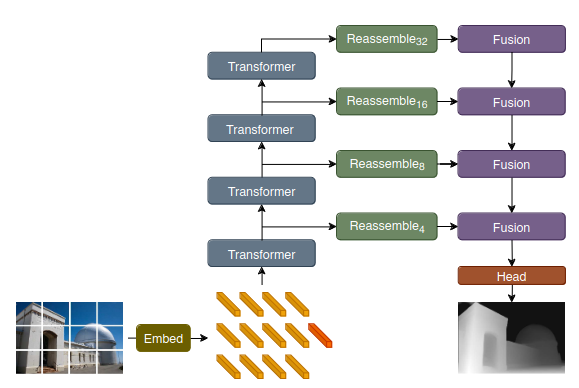
\includegraphics[scale=0.5]{midas}
    \end{figure}
\end{frame}

\begin{frame}
    \frametitle{Получение карты абсолютной глубины}
    Модель Midas строит по изображению карту относительной глубины $M_r$. Преобразуем её в карту абсолютной глубины $M_a$.

    Зная точное расстояние $d_0$ до одной из точек $(x_0, y_0)$ на изображении можно масштабировать карту относительной глубины следующим образом:
    $$ M_a = c \cdot M_r, $$

    где $c = \frac{d}{M_r[x_0, y_0]}$
\end{frame}

\begin{frame}
    \frametitle{Уточнение карты абсолютной глубины}
    Пусть мы знаем расстояния $d = \left(d_0, \dots, d_{k - 1}\right)$ до точек $A = \left((x_0, y_0), \dots, (x_{k - 1}, y_{k - 1})\right)$.

    Определим функцию ошибки приближения следующим образом:
    $$ L_{(d, A)}(c) = \sum\limits_{i = 0}^{k - 1} \left(c \cdot M_r[x_i, y_i] - d_i\right)^2 $$

    Методом наименьших квадратов найдём такое $c$, при котором достигается минимум $L(c)$.
\end{frame}

\begin{frame}
    \frametitle{Примеры работы алгоритма проверки принадлежности опасной зоне}
    \begin{figure}
        \begin{minipage}[!h]{0.49\linewidth}
            \centering
            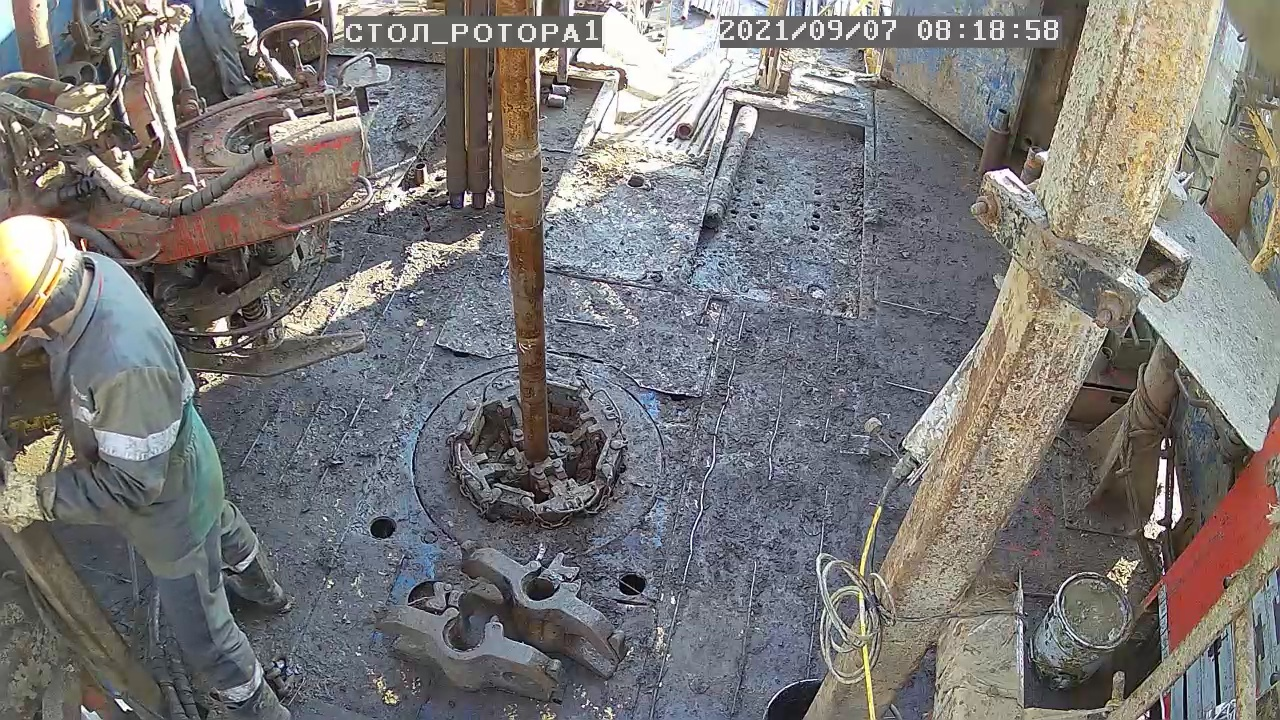
\includegraphics[width=1.0\textwidth,keepaspectratio]{example_1_image}
        \end{minipage}
        \hfill
        \begin{minipage}[!h]{0.49\linewidth}
            \centering
            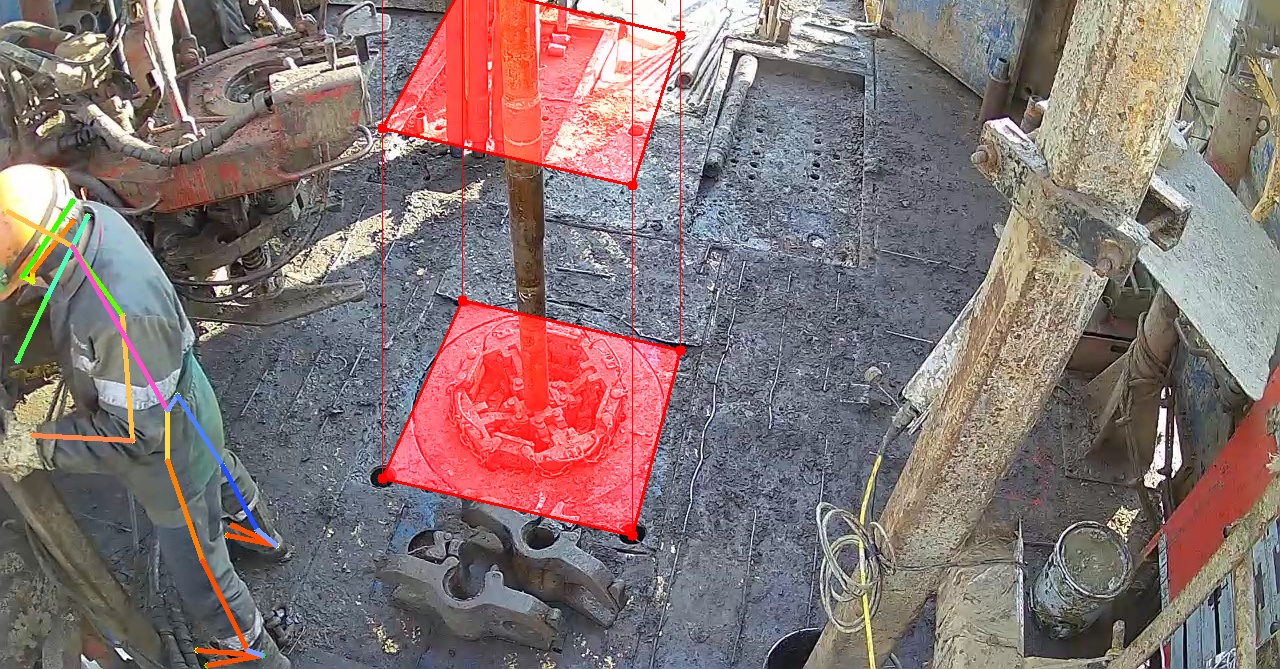
\includegraphics[width=1.08\textwidth,keepaspectratio]{example_1_highlighted}
        \end{minipage}
        \caption{Рабочий в СИЗ не в опасной зоне}
    \end{figure}
\end{frame}

\begin{frame}
    \frametitle{Примеры работы алгоритма проверки принадлежности опасной зоне}
    \begin{figure}
        \begin{minipage}[!h]{0.49\linewidth}
            \centering
            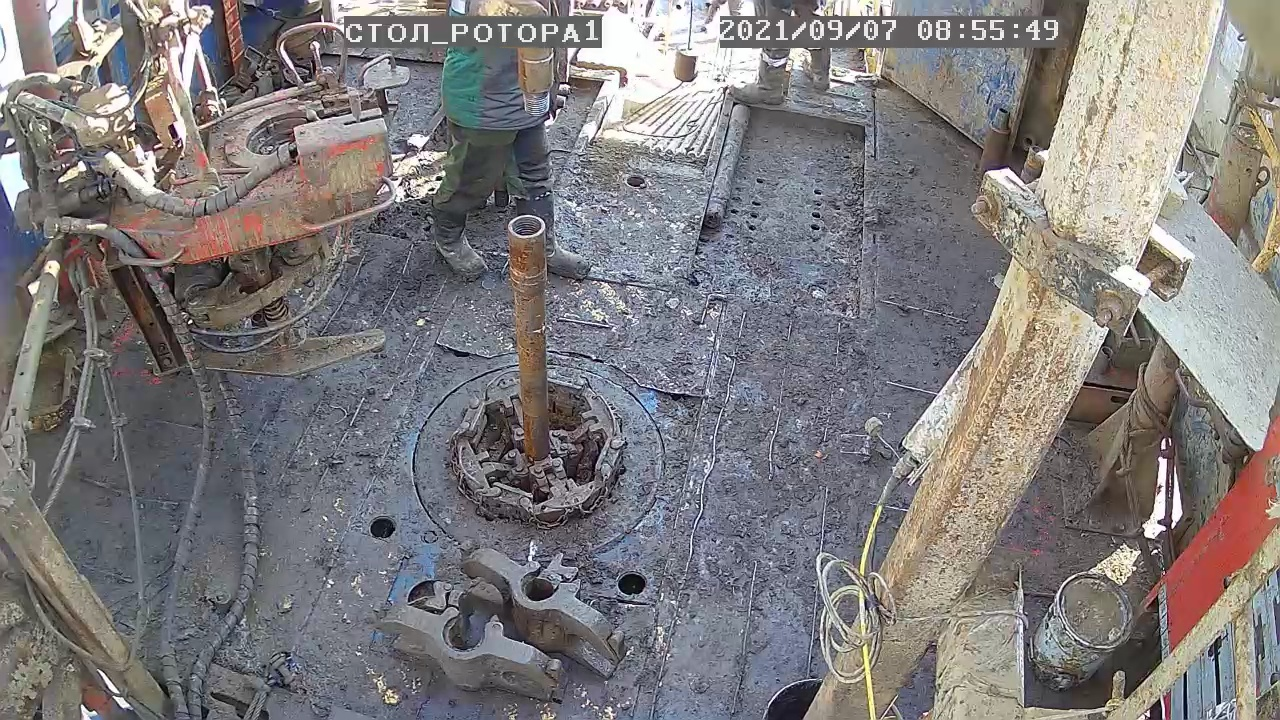
\includegraphics[width=1.0\textwidth,keepaspectratio]{example_2_image}
        \end{minipage}
        \hfill
        \begin{minipage}[!h]{0.49\linewidth}
            \centering
            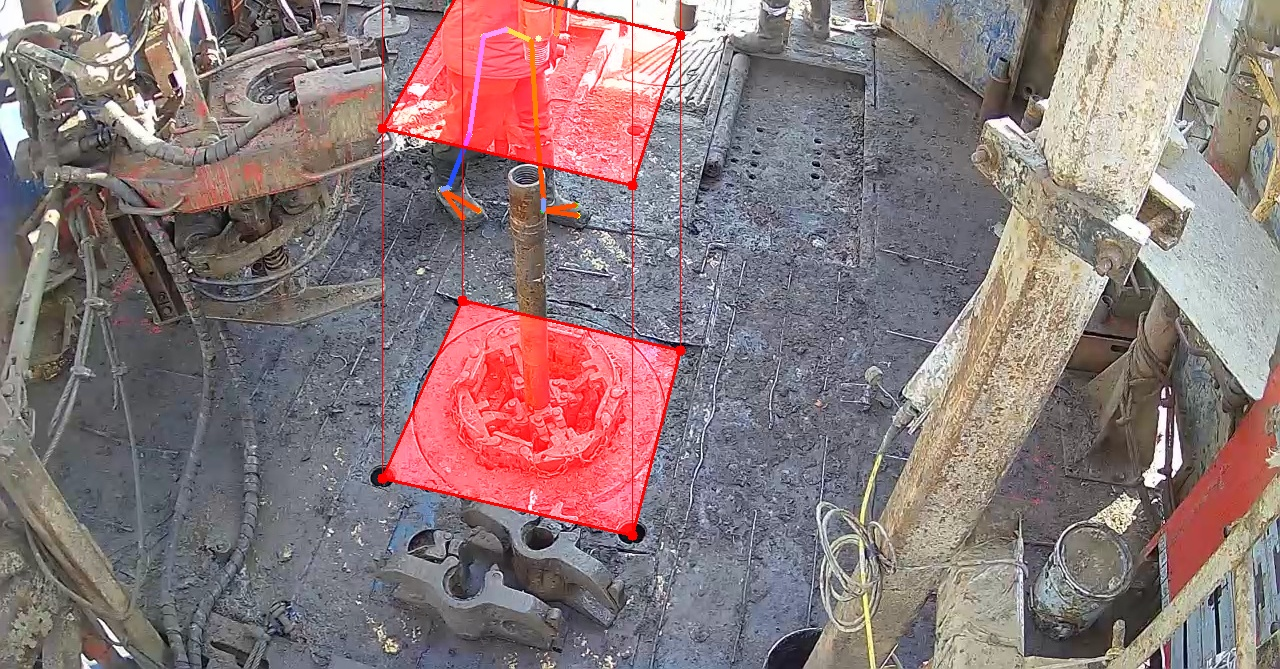
\includegraphics[width=1.08\textwidth,keepaspectratio]{example_2_highlighted}
        \end{minipage}
        \caption{Рабочий в СИЗ за опасной зоной}
    \end{figure}
\end{frame}

\begin{frame}
    \frametitle{Примеры работы алгоритма проверки принадлежности опасной зоне}
    \begin{figure}
        \begin{minipage}[!h]{0.49\linewidth}
            \centering
            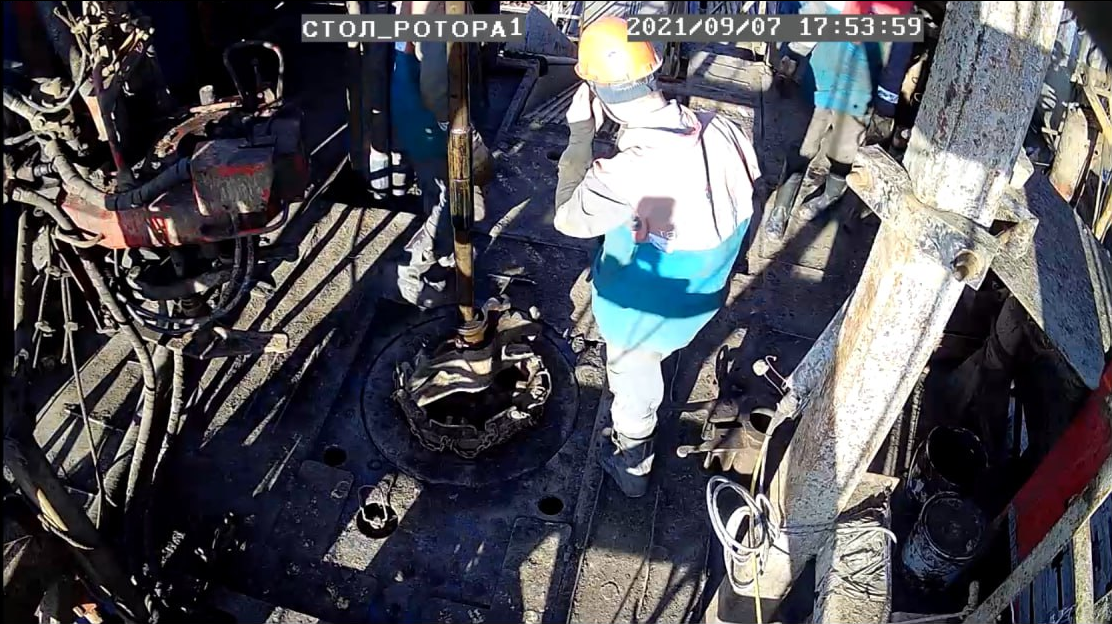
\includegraphics[width=1.0\textwidth,keepaspectratio]{example_3_image}
        \end{minipage}
        \hfill
        \begin{minipage}[!h]{0.49\linewidth}
            \centering
            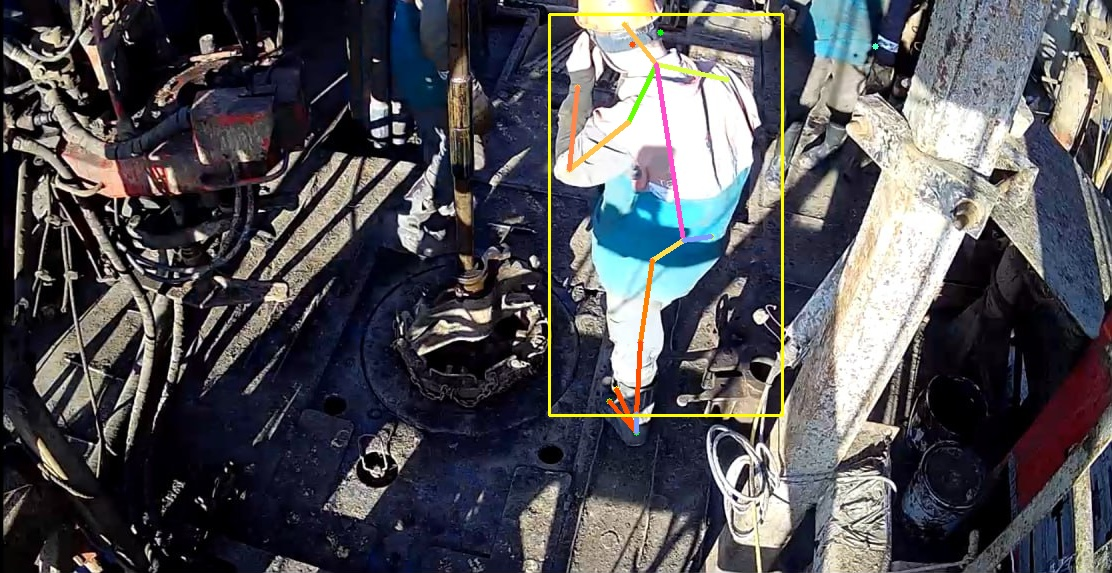
\includegraphics[width=1.08\textwidth,keepaspectratio]{example_3_highlighted}
        \end{minipage}
        \caption{Рабочий без СИЗ в опасной зоне}
    \end{figure}
\end{frame}